\chapter{ANTARMUKA \textit{DASHBOARD}}
\label{chap:lampiran-b}

Lampiran ini menyajikan tampilan lengkap antarmuka \textit{dashboard Smart Waste Bin}
yang telah diimplementasikan dan di-\textit{deploy} pada \textit{platform} Vercel.

\begin{figure}[H]
  \caption{Tampilan Keseluruhan \textit{Dashboard Smart Waste Bin}}
  \label{fig:lamp-dashboard-full}
  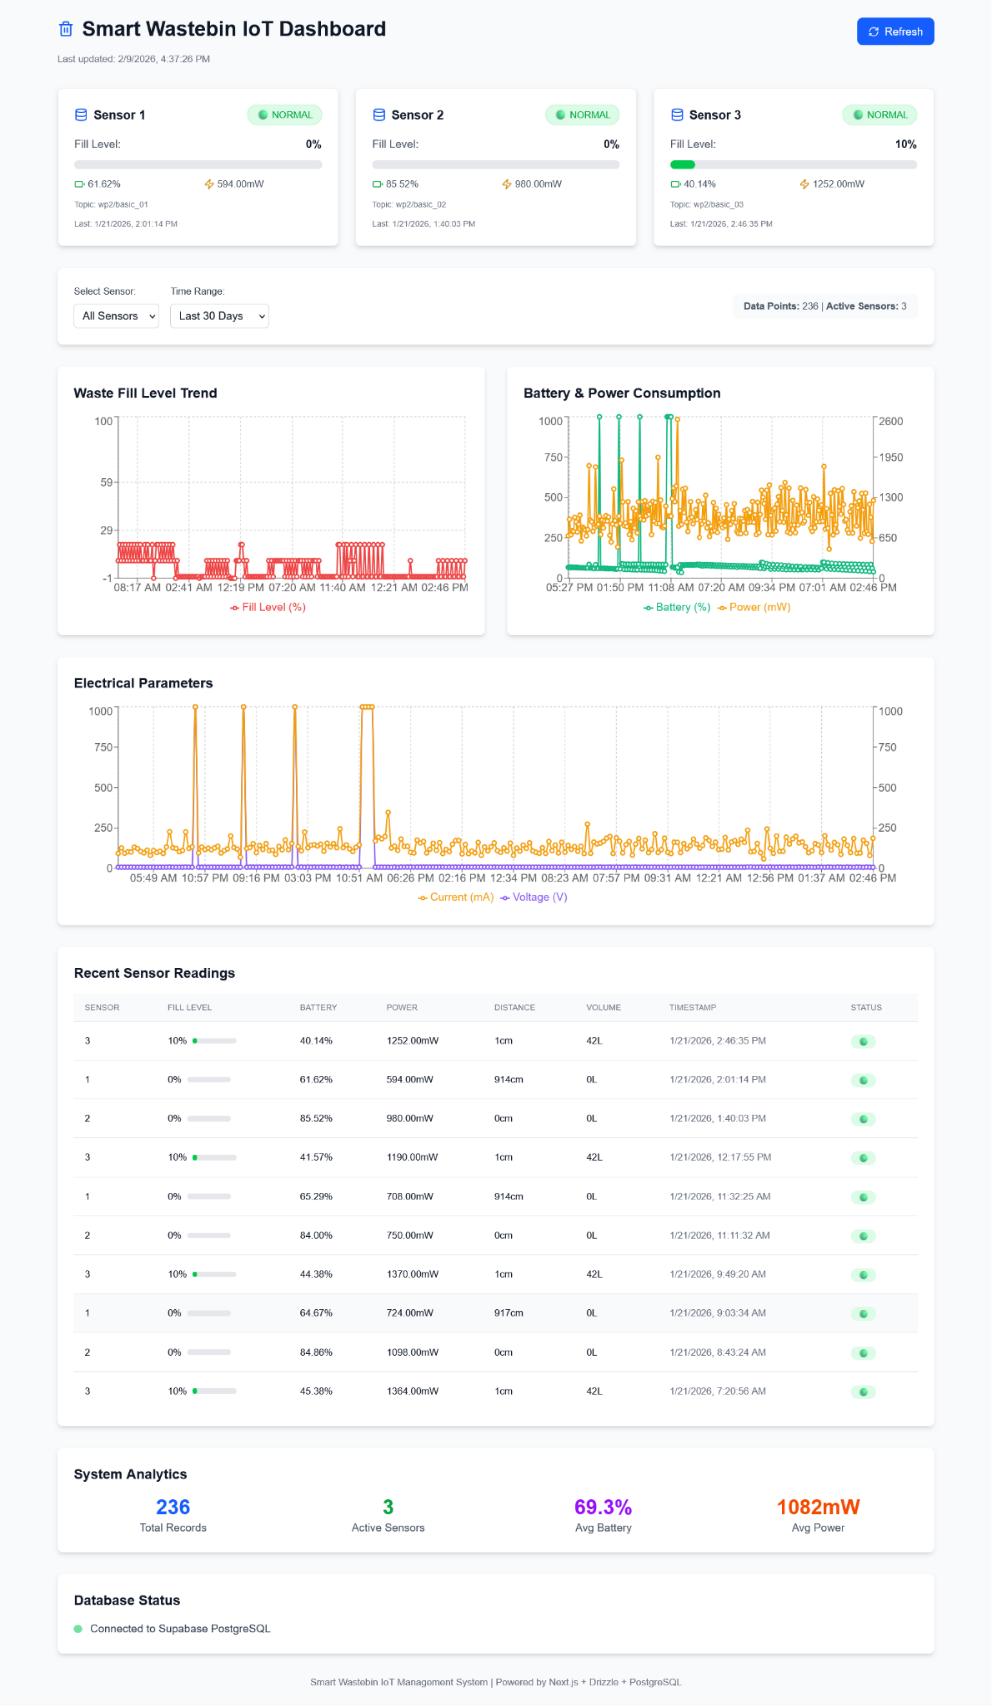
\includegraphics[width=0.85\textwidth]{images/dashboard-full.png}
  % RENAME: image21.png → dashboard-full.png
\end{figure}

\begin{figure}[H]
  \caption{\textit{Header Section Dashboard}}
  \label{fig:lamp-header}
  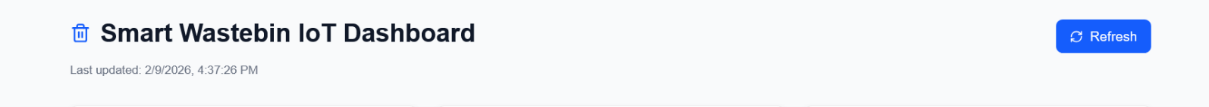
\includegraphics[width=\textwidth]{images/dashboard-header.png}
  % RENAME: image22.png → dashboard-header.png
\end{figure}

\begin{figure}[H]
  \caption{\textit{Sensor Status Cards}}
  \label{fig:lamp-cards}
  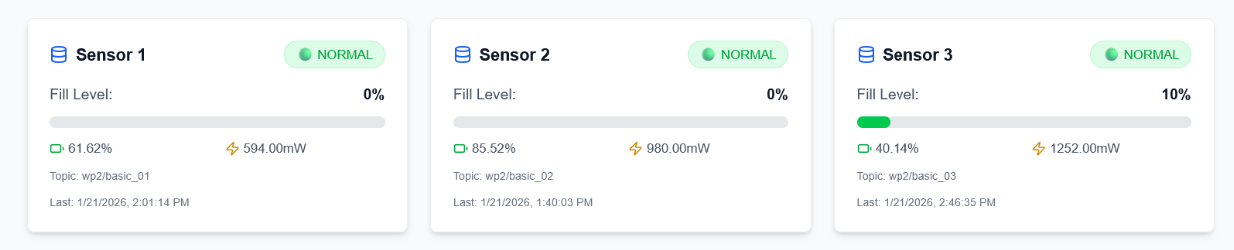
\includegraphics[width=\textwidth]{images/dashboard-cards.png}
  % RENAME: image23.png → dashboard-cards.png
\end{figure}

\begin{figure}[H]
  \caption{\textit{Control Panel}}
  \label{fig:lamp-control}
  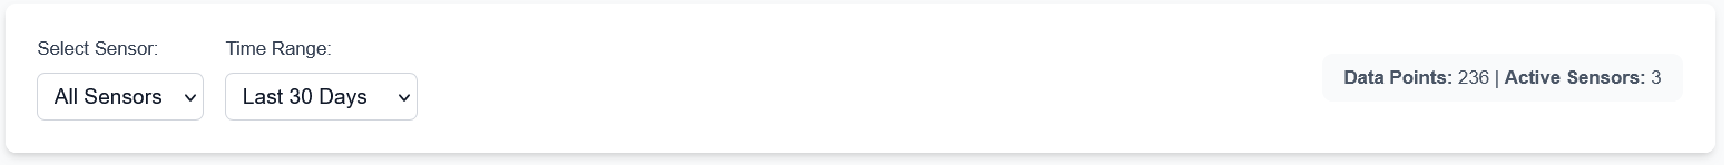
\includegraphics[width=\textwidth]{images/dashboard-control.png}
  % RENAME: image24.png → dashboard-control.png
\end{figure}

\begin{figure}[H]
  \caption{Visualisasi Data}
  \label{fig:lamp-chart}
  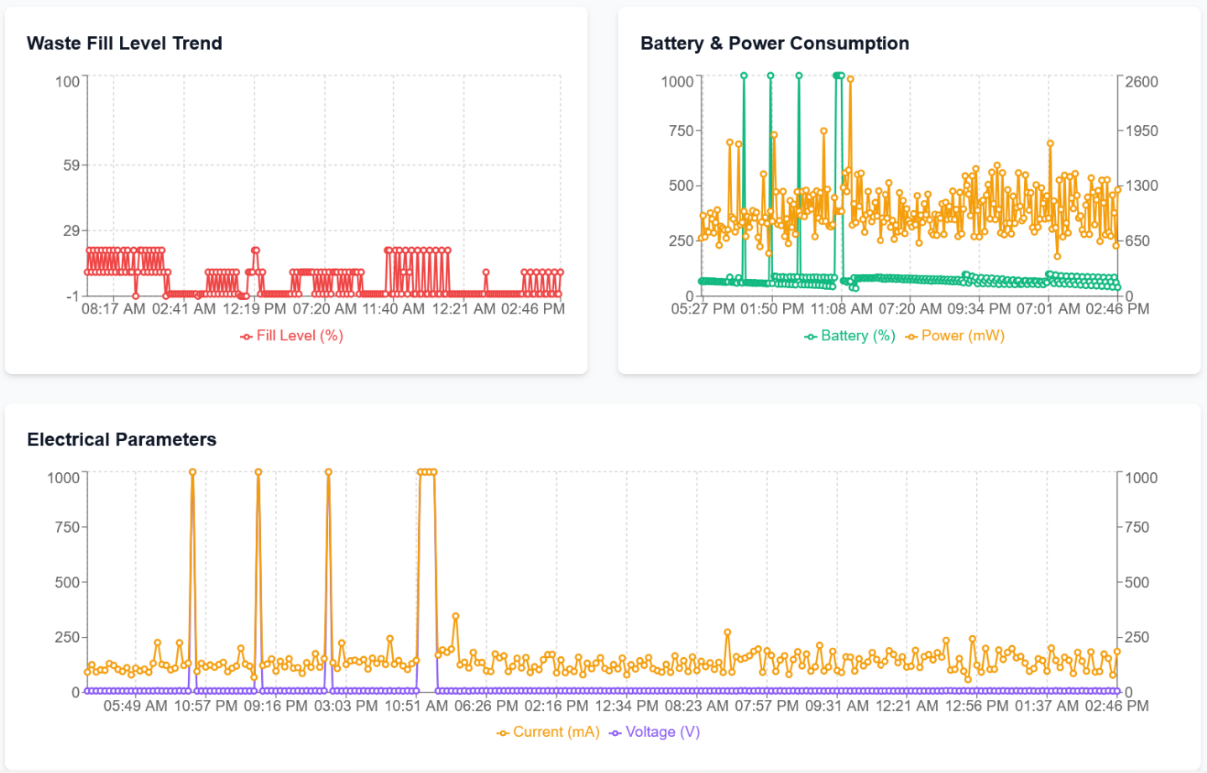
\includegraphics[width=\textwidth]{images/dashboard-chart.png}
  % RENAME: image25.png → dashboard-chart.png
\end{figure}

\begin{figure}[H]
  \caption{\textit{Recent Sensor Readings}}
  \label{fig:lamp-readings}
  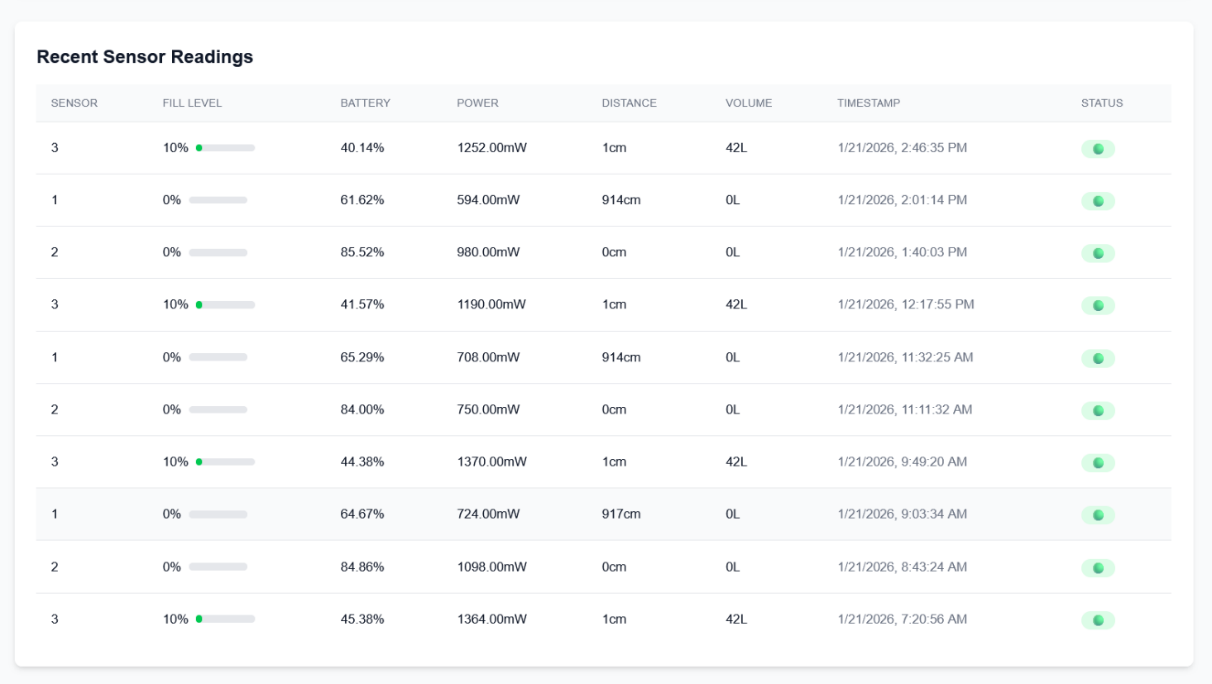
\includegraphics[width=\textwidth]{images/dashboard-readings.png}
  % RENAME: image26.png → dashboard-readings.png
\end{figure}

\begin{figure}[H]
  \caption{\textit{System Analytics}}
  \label{fig:lamp-analytics}
  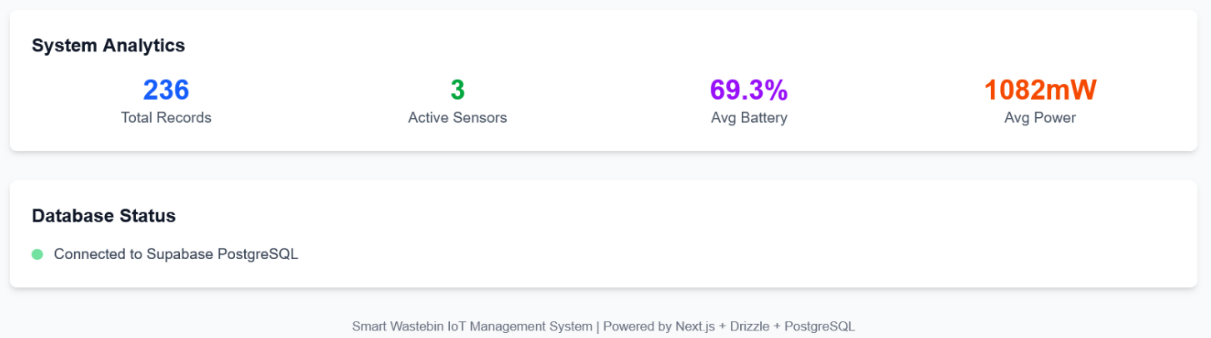
\includegraphics[width=\textwidth]{images/dashboard-analytics.png}
  % RENAME: image27.png → dashboard-analytics.png
\end{figure}